\chapter{Stand der Technik}
\label{ch:StandDerTechnik}

Forschungen über Kollaborative Engineering Tools gibt es direkt keine. Die Forschungen können aber in zwei Bereiche aufgeteilt werden. Zum einen gibt es das virtuelle Engineering und zum anderen die Zusammenarbeit in der virtuellen Realität.

\section{Virtuelles Engineering}

Im Bereich des virtuellen Engineerings gibt es verschiedene Forschungen welche sich mit dem Thema Zusammenbau und insbesondere Kollision zwischen den Elementen beschäftigen.
Eine Arbeit befasst sich mit der Berechnung der Kollisionen zwischen Elementen welche aus einem CAD Model importiert wurden. (\cite{tching_interactive_2010})
Wie in Abbildung \ref{fig:LossOfAccuracy} zu sehen ist, nimmt die Genauigkeit der importierten Modelle aber ab und somit verhalten sich die beiden Objekte bei der Kollision miteinander nicht mehr flüssig.

\begin{figure}[h!]
	\centering
	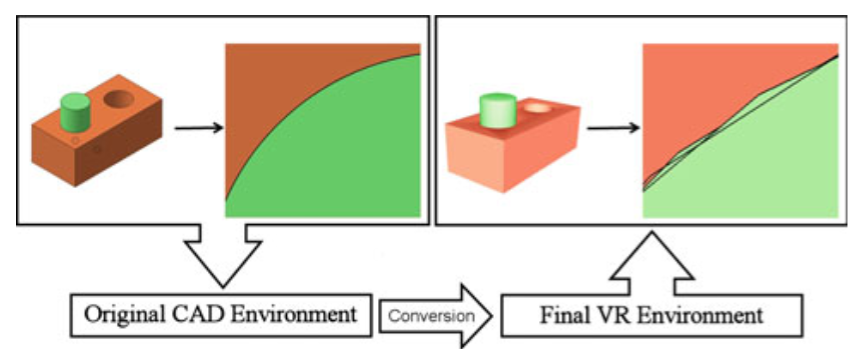
\includegraphics[keepaspectratio,width=0.6\linewidth]{CollisionDetection.png}
	\caption{Verlust der Genauigkeit bei der Konvertierung eines CAD-Models zu VR}
	\label{fig:LossOfAccuracy}
\end{figure}

\noindent VADE (\cite{noauthor_vade:_nodate}) ist eine virtuelle Assembly Design-Umgebung. In dieser werden je nach Situation die Freiheitsgrade der Bewegung des Bauteils eingeschränkt um das Zusammenbauen diverser Bauteile zu erleichtern. 
In der Abbildung \ref{fig:VADEAssembly} kann das Bauteil in der rechten Hand nur auf den hervorgehobenen Achsen bewegt werden. \\

\begin{figure}[h!]
	\centering
	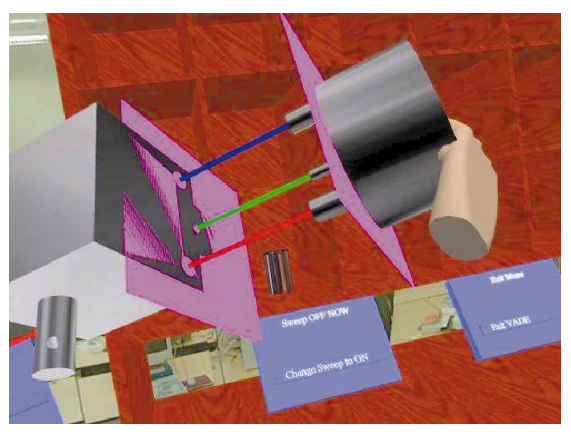
\includegraphics[keepaspectratio,width=0.4\linewidth]{VADE_PartsAssembly.png}
	\caption{Einschränkungen beim Zusammenbau in VADE}
	\label{fig:VADEAssembly}
\end{figure}

\noindent In der Arbeit "Virtual reality and augmented reality as a training tool for assembly tasks" (\cite{boud_virtual_1999}) wurde bereits 1999 untersucht ob das virtuelle Assembly Training einen Mehrwert gegenüber dem Training mit normalen Modellen in der realen Welt bringt. Nach ihrer Aussage, hat das virtuelle Training Zukunft, da das Training bereits gestartet werden kann, ohne dass ein Prototyp vorhanden ist. Aktuell sei die Technik im Bereich der virtuellen Realität aber noch nicht bereit dafür. 

\section{Zusammenarbeit in der virtuellen Realität}
Für die Zusammenarbeit in der virtuellen Realität gibt es drei Stufen. Die erste Stufe definiert wie sich die Benutzer in der virtuellen Realität wahrnehmen. Die zweite Stufe ist die alleinige Manipulation in der virtuellen Umgebung und die dritte Stufe die gleichzeitige Manipulation eines Objektes in dieser virtuellen Umgebung. 

% TODO: Collaborative Virtual Environments

\subsection{Collaborative User Interaction}
Um eine gleichzeitige Interaktion am selben Objekt zu ermöglichen hat Márcio S. Pinho bereits 2002 (\cite{pinho_cooperative_2002}) eine Variante beschrieben, bei welcher die Freiheitsgrade der Benutzer separiert werden. Bei einem Würfel wäre das zum Beispiel wie folgt aufgeteilt. Ein Benutzer rotiert den Würfel während der andere Benutzer den Würfel in der virtuellen Welt bewegen kann. \\
 
\noindent Eine andere Arbeit befasste sich ebenfalls mit der gleichzeitigen Manipulation eines Objektes und beschreibt ein Lösungsansatz, bei welchem der Mittelwert aller Nutzer genommen und auf das Objekt übertragen wird.(\cite{ruddle_symmetric_2002}) \\
 
\noindent Um der Realität so nahe wie möglich zu kommen gibt es diverse Arbeiten, welche sich damit beschäftigen getrackte Objekte in der realen Welt zu verwenden um virtuelle Objekte zu manipulieren. (\cite{he_physhare:_2017}) (\cite{podkosova_immersivedeck:_2016}) In der realen Welt befindet sich ein abstrahiertes Objekt welches ein Objekt in der virtuellen Realität darstellt. Wollen mehrere Nutzer dieses Objekt manipulieren greifen sie das Objekt in der realen Welt und haben so ein natürliches Verhalten. Für diese Variante müssen sich aber alle Nutzer im selben Raum befinden.
 
\subsection{User Representation}

Wie wird ein Benutzer einem anderen Benutzer in der virtuellen Realität dargestellt? 
Für viele Anwendungen reicht es den Kopf und die Hände des anderen Nutzers zu sehen.
3D-Körper gibt es in verschiedenen Variationen. Menschliche Körper besitzen mehrere hundert Muskeln und Gelenke. Sowas in VR umzusetzen ist schwierig.
Heutzutage gibt es Systeme, um das Gesicht und den Körper in der virtuellen Realität möglichst real zu animieren. Die Arbeit «Interactive Virtual Humans in Real-Time Virtual Environment» gibt eine gute Übersicht darüber. (Interactive Virtual Humans in Real-Time Virtual Environment)


\subsection{Communication Among people}

Kommunikation direkt via Audio-Aufnahmen integriert in die Applikation oder die Kommunikation mit der anderen Person direkt falls man sich im gleichen Raum befindet.
-	Synchrone oder asynchrone Kommunikation
Körpersprache wie zB. das Zeigen mit den Händen oder die Orientation des Kopfes
